\section{مقدمه}

\begin{frame}[standout]
چند تعریف...
\end{frame}
\begin{frame}{تانسور}
\begin{center}
	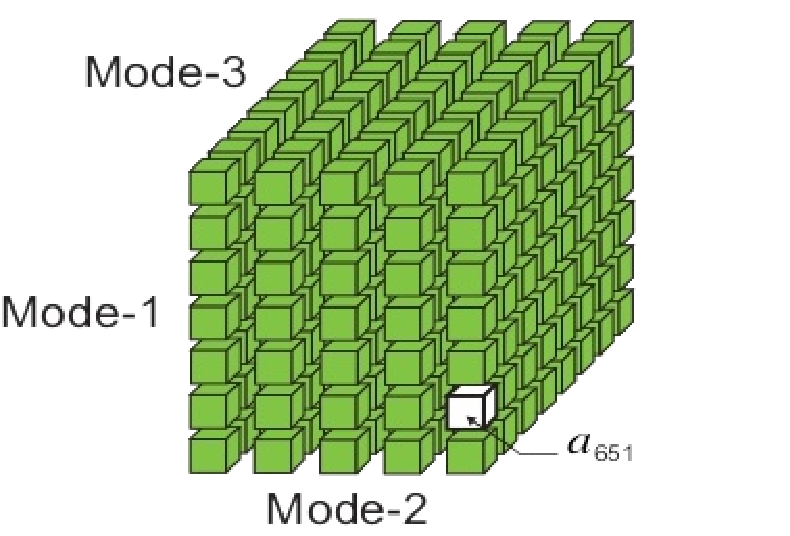
\includegraphics[width=0.5\textwidth]{img/ok/tensor3d.pdf}
\end{center}
\begin{center}
	تانسور سه بعدی
\end{center}
\end{frame}
\begin{frame}
\begin{center}
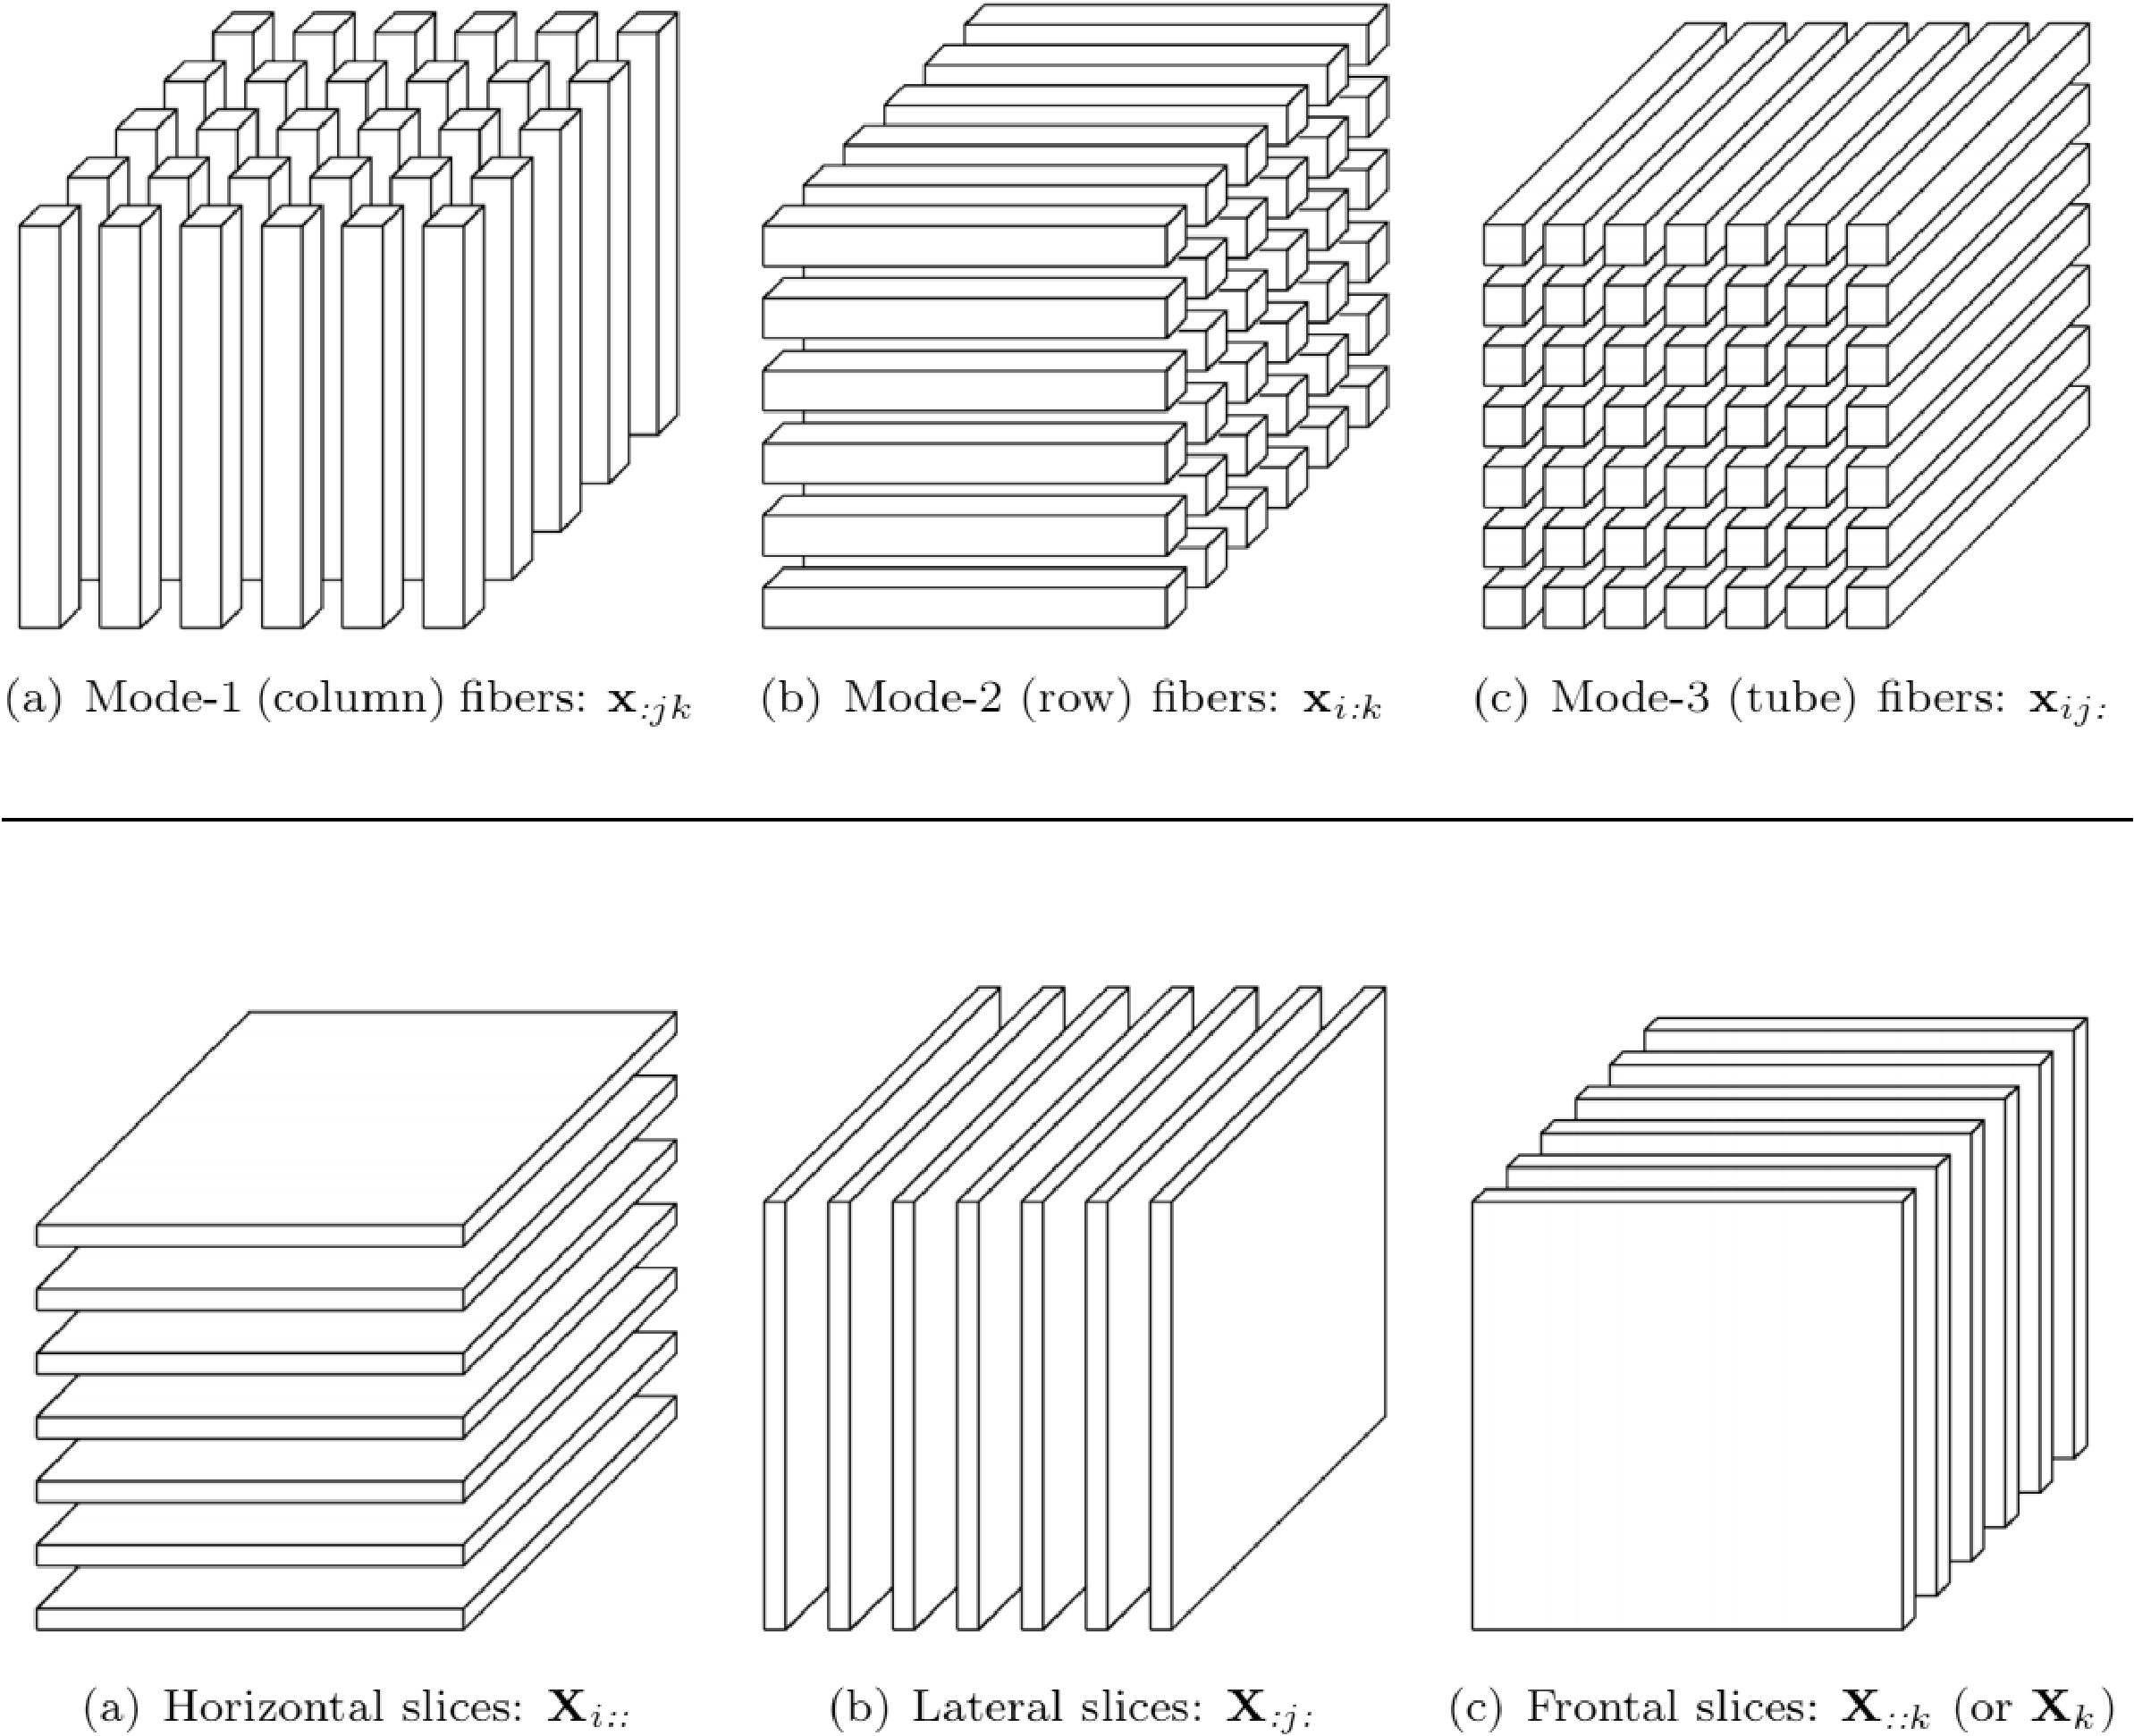
\includegraphics[width=0.9\textwidth]{img/ok/slice.pdf}
\end{center}
\end{frame}
\begin{frame}
\small{
\begin{columns}[T,onlytextwidth]
	\column{1\textwidth}	
	\metroset{block=fill}
	\begin{exampleblock}{ترانهاده ماتریس}
		ترانهاده تانسور 3-بعدی
		$\mathcal{A}\in\mathbb{R}^{n_1\times n_2\times n_3}$
		را با $\mathcal{A}^T$ نشان داده که یک تانسور با ابعاد
		$n_1\times n_2\times n_3$
		است.
		
	\end{exampleblock}\pause
	\begin{alertblock}{تانسور همانی}
		یک تانسور سه بعدی صفر را که تنها در اسلایس اولی ماتریس همانی وجود دارد را تانسور همانی گوییم.
	\end{alertblock}\pause
	\begin{block}{ضرب داخلی}
	ضرب داخلی	دو تانسور هم‌اندازه
		$\mathcal{X},\mathcal{Y}\in \mathbb{R}^{I_1\times\cdots \times I_N}$
		به‌صورت زیر تعریف می‌شود.
		\begin{center}
			\begin{tabular}{ccc}
			&$
			<\mathcal{X},\mathcal{Y}>=\displaystyle\sum_{i_1=1}^{I_1}\cdots \sum_{i_N=1}^{I_N}
			x_{i_1,i_2,\cdots,i_N}y_{i_1,i_2,\cdots,i_N}
			$&
		\end{tabular}
		\end{center}		
	\end{block}
\end{columns}
}
\end{frame}

